% Created by tikzDevice version 0.10.1 on 2017-10-30 17:28:41
% !TEX encoding = UTF-8 Unicode
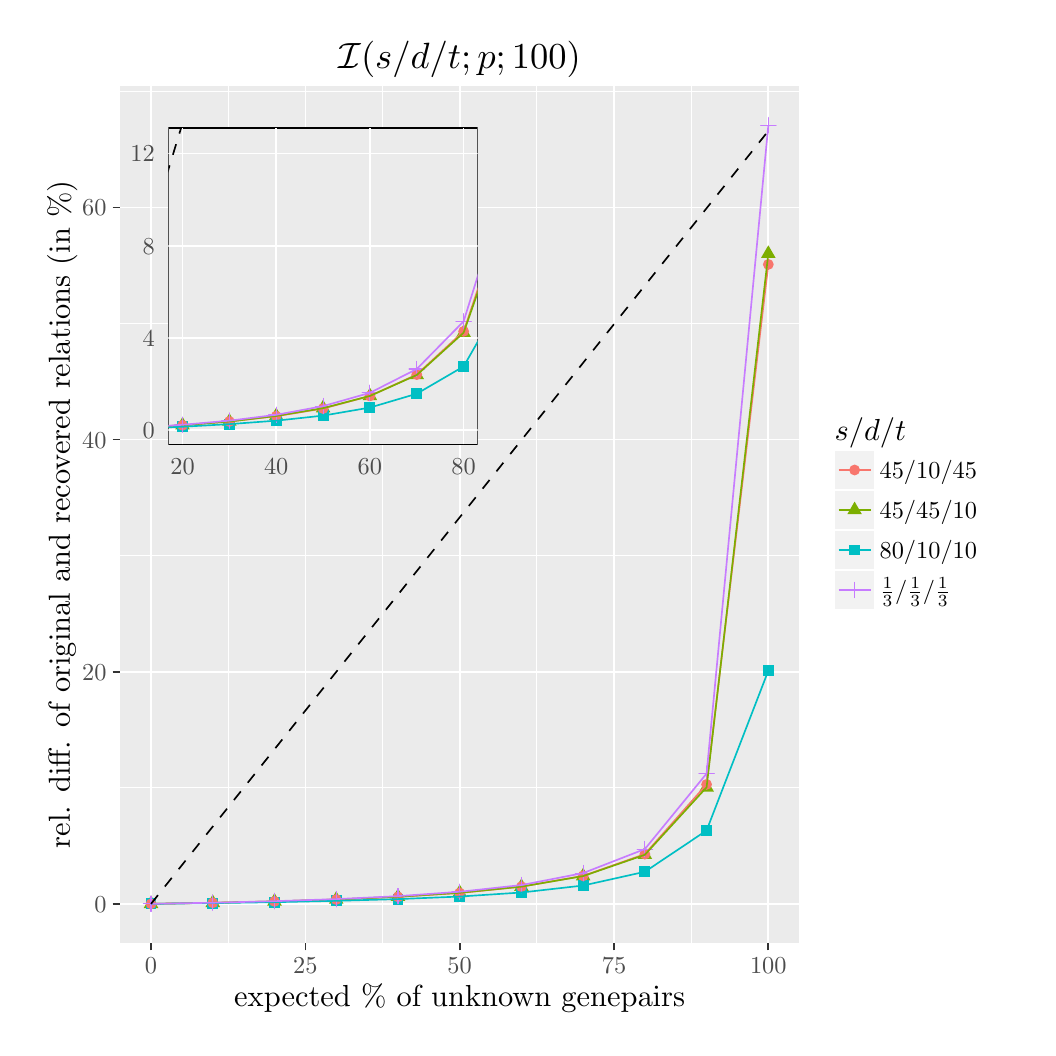
\begin{tikzpicture}[x=1pt,y=1pt]
\definecolor{fillColor}{RGB}{255,255,255}
\path[use as bounding box,fill=fillColor,fill opacity=0.00] (0,0) rectangle (361.35,361.35);
\begin{scope}
\path[clip] (  0.00,  0.00) rectangle (361.35,361.35);
\definecolor{drawColor}{RGB}{255,255,255}
\definecolor{fillColor}{RGB}{255,255,255}

\path[draw=drawColor,line width= 0.6pt,line join=round,line cap=round,fill=fillColor] (  0.00,  0.00) rectangle (361.35,361.35);
\end{scope}
\begin{scope}
\path[clip] ( 33.42, 30.69) rectangle (278.78,340.16);
\definecolor{fillColor}{gray}{0.92}

\path[fill=fillColor] ( 33.42, 30.69) rectangle (278.78,340.16);
\definecolor{drawColor}{RGB}{255,255,255}

\path[draw=drawColor,line width= 0.3pt,line join=round] ( 33.42, 86.69) --
	(278.78, 86.69);

\path[draw=drawColor,line width= 0.3pt,line join=round] ( 33.42,170.55) --
	(278.78,170.55);

\path[draw=drawColor,line width= 0.3pt,line join=round] ( 33.42,254.42) --
	(278.78,254.42);

\path[draw=drawColor,line width= 0.3pt,line join=round] ( 33.42,338.28) --
	(278.78,338.28);

\path[draw=drawColor,line width= 0.3pt,line join=round] ( 72.46, 30.69) --
	( 72.46,340.16);

\path[draw=drawColor,line width= 0.3pt,line join=round] (128.22, 30.69) --
	(128.22,340.16);

\path[draw=drawColor,line width= 0.3pt,line join=round] (183.98, 30.69) --
	(183.98,340.16);

\path[draw=drawColor,line width= 0.3pt,line join=round] (239.75, 30.69) --
	(239.75,340.16);

\path[draw=drawColor,line width= 0.6pt,line join=round] ( 33.42, 44.75) --
	(278.78, 44.75);

\path[draw=drawColor,line width= 0.6pt,line join=round] ( 33.42,128.62) --
	(278.78,128.62);

\path[draw=drawColor,line width= 0.6pt,line join=round] ( 33.42,212.48) --
	(278.78,212.48);

\path[draw=drawColor,line width= 0.6pt,line join=round] ( 33.42,296.35) --
	(278.78,296.35);

\path[draw=drawColor,line width= 0.6pt,line join=round] ( 44.58, 30.69) --
	( 44.58,340.16);

\path[draw=drawColor,line width= 0.6pt,line join=round] (100.34, 30.69) --
	(100.34,340.16);

\path[draw=drawColor,line width= 0.6pt,line join=round] (156.10, 30.69) --
	(156.10,340.16);

\path[draw=drawColor,line width= 0.6pt,line join=round] (211.87, 30.69) --
	(211.87,340.16);

\path[draw=drawColor,line width= 0.6pt,line join=round] (267.63, 30.69) --
	(267.63,340.16);
\definecolor{fillColor}{RGB}{124,174,0}

\path[fill=fillColor] ( 44.58, 47.80) --
	( 47.22, 43.23) --
	( 41.93, 43.23) --
	cycle;

\path[fill=fillColor] ( 66.88, 48.18) --
	( 69.52, 43.60) --
	( 64.24, 43.60) --
	cycle;

\path[fill=fillColor] ( 89.19, 48.69) --
	( 91.83, 44.11) --
	( 86.54, 44.11) --
	cycle;

\path[fill=fillColor] (111.49, 49.36) --
	(114.13, 44.78) --
	(108.85, 44.78) --
	cycle;

\path[fill=fillColor] (133.80, 50.37) --
	(136.44, 45.80) --
	(131.15, 45.80) --
	cycle;

\path[fill=fillColor] (156.10, 51.79) --
	(158.75, 47.21) --
	(153.46, 47.21) --
	cycle;

\path[fill=fillColor] (178.41, 54.01) --
	(181.05, 49.43) --
	(175.77, 49.43) --
	cycle;

\path[fill=fillColor] (200.71, 57.82) --
	(203.36, 53.24) --
	(198.07, 53.24) --
	cycle;

\path[fill=fillColor] (223.02, 65.53) --
	(225.66, 60.95) --
	(220.38, 60.95) --
	cycle;

\path[fill=fillColor] (245.32, 89.90) --
	(247.97, 85.33) --
	(242.68, 85.33) --
	cycle;

\path[fill=fillColor] (267.63,282.72) --
	(270.27,278.14) --
	(264.99,278.14) --
	cycle;
\definecolor{fillColor}{RGB}{0,191,196}

\path[fill=fillColor] ( 42.61, 42.79) --
	( 46.54, 42.79) --
	( 46.54, 46.72) --
	( 42.61, 46.72) --
	cycle;

\path[fill=fillColor] ( 64.92, 43.05) --
	( 68.84, 43.05) --
	( 68.84, 46.98) --
	( 64.92, 46.98) --
	cycle;

\path[fill=fillColor] ( 87.22, 43.39) --
	( 91.15, 43.39) --
	( 91.15, 47.31) --
	( 87.22, 47.31) --
	cycle;

\path[fill=fillColor] (109.53, 43.87) --
	(113.45, 43.87) --
	(113.45, 47.79) --
	(109.53, 47.79) --
	cycle;

\path[fill=fillColor] (131.84, 44.50) --
	(135.76, 44.50) --
	(135.76, 48.42) --
	(131.84, 48.42) --
	cycle;

\path[fill=fillColor] (154.14, 45.42) --
	(158.06, 45.42) --
	(158.06, 49.34) --
	(154.14, 49.34) --
	cycle;

\path[fill=fillColor] (176.45, 46.88) --
	(180.37, 46.88) --
	(180.37, 50.80) --
	(176.45, 50.80) --
	cycle;

\path[fill=fillColor] (198.75, 49.40) --
	(202.68, 49.40) --
	(202.68, 53.32) --
	(198.75, 53.32) --
	cycle;

\path[fill=fillColor] (221.06, 54.36) --
	(224.98, 54.36) --
	(224.98, 58.29) --
	(221.06, 58.29) --
	cycle;

\path[fill=fillColor] (243.36, 69.29) --
	(247.29, 69.29) --
	(247.29, 73.21) --
	(243.36, 73.21) --
	cycle;

\path[fill=fillColor] (265.67,127.02) --
	(269.59,127.02) --
	(269.59,130.95) --
	(265.67,130.95) --
	cycle;
\definecolor{fillColor}{RGB}{248,118,109}

\path[fill=fillColor] ( 44.58, 44.75) circle (  1.96);

\path[fill=fillColor] ( 66.88, 45.11) circle (  1.96);

\path[fill=fillColor] ( 89.19, 45.62) circle (  1.96);

\path[fill=fillColor] (111.49, 46.31) circle (  1.96);

\path[fill=fillColor] (133.80, 47.27) circle (  1.96);

\path[fill=fillColor] (156.10, 48.66) circle (  1.96);

\path[fill=fillColor] (178.41, 50.95) circle (  1.96);

\path[fill=fillColor] (200.71, 54.85) circle (  1.96);

\path[fill=fillColor] (223.02, 62.72) circle (  1.96);

\path[fill=fillColor] (245.32, 87.90) circle (  1.96);

\path[fill=fillColor] (267.63,275.80) circle (  1.96);
\definecolor{drawColor}{RGB}{199,124,255}

\path[draw=drawColor,line width= 0.4pt,line join=round,line cap=round] ( 41.80, 44.75) -- ( 47.35, 44.75);

\path[draw=drawColor,line width= 0.4pt,line join=round,line cap=round] ( 44.58, 41.98) -- ( 44.58, 47.53);

\path[draw=drawColor,line width= 0.4pt,line join=round,line cap=round] ( 64.11, 45.15) -- ( 69.66, 45.15);

\path[draw=drawColor,line width= 0.4pt,line join=round,line cap=round] ( 66.88, 42.38) -- ( 66.88, 47.93);

\path[draw=drawColor,line width= 0.4pt,line join=round,line cap=round] ( 86.41, 45.71) -- ( 91.96, 45.71);

\path[draw=drawColor,line width= 0.4pt,line join=round,line cap=round] ( 89.19, 42.94) -- ( 89.19, 48.49);

\path[draw=drawColor,line width= 0.4pt,line join=round,line cap=round] (108.72, 46.46) -- (114.27, 46.46);

\path[draw=drawColor,line width= 0.4pt,line join=round,line cap=round] (111.49, 43.68) -- (111.49, 49.23);

\path[draw=drawColor,line width= 0.4pt,line join=round,line cap=round] (131.02, 47.52) -- (136.57, 47.52);

\path[draw=drawColor,line width= 0.4pt,line join=round,line cap=round] (133.80, 44.75) -- (133.80, 50.30);

\path[draw=drawColor,line width= 0.4pt,line join=round,line cap=round] (153.33, 49.11) -- (158.88, 49.11);

\path[draw=drawColor,line width= 0.4pt,line join=round,line cap=round] (156.10, 46.33) -- (156.10, 51.88);

\path[draw=drawColor,line width= 0.4pt,line join=round,line cap=round] (175.63, 51.53) -- (181.18, 51.53);

\path[draw=drawColor,line width= 0.4pt,line join=round,line cap=round] (178.41, 48.75) -- (178.41, 54.30);

\path[draw=drawColor,line width= 0.4pt,line join=round,line cap=round] (197.94, 55.86) -- (203.49, 55.86);

\path[draw=drawColor,line width= 0.4pt,line join=round,line cap=round] (200.71, 53.08) -- (200.71, 58.63);

\path[draw=drawColor,line width= 0.4pt,line join=round,line cap=round] (220.24, 64.54) -- (225.79, 64.54);

\path[draw=drawColor,line width= 0.4pt,line join=round,line cap=round] (223.02, 61.76) -- (223.02, 67.31);

\path[draw=drawColor,line width= 0.4pt,line join=round,line cap=round] (242.55, 91.82) -- (248.10, 91.82);

\path[draw=drawColor,line width= 0.4pt,line join=round,line cap=round] (245.32, 89.04) -- (245.32, 94.59);

\path[draw=drawColor,line width= 0.4pt,line join=round,line cap=round] (264.85,326.09) -- (270.40,326.09);

\path[draw=drawColor,line width= 0.4pt,line join=round,line cap=round] (267.63,323.32) -- (267.63,328.87);
\definecolor{drawColor}{RGB}{248,118,109}

\path[draw=drawColor,line width= 0.6pt,line join=round] ( 44.58, 44.75) --
	( 66.88, 45.11) --
	( 89.19, 45.62) --
	(111.49, 46.31) --
	(133.80, 47.27) --
	(156.10, 48.66) --
	(178.41, 50.95) --
	(200.71, 54.85) --
	(223.02, 62.72) --
	(245.32, 87.90) --
	(267.63,275.80);
\definecolor{drawColor}{RGB}{124,174,0}

\path[draw=drawColor,line width= 0.6pt,line join=round] ( 44.58, 44.75) --
	( 66.88, 45.13) --
	( 89.19, 45.63) --
	(111.49, 46.30) --
	(133.80, 47.32) --
	(156.10, 48.74) --
	(178.41, 50.96) --
	(200.71, 54.77) --
	(223.02, 62.47) --
	(245.32, 86.85) --
	(267.63,279.67);
\definecolor{drawColor}{RGB}{0,191,196}

\path[draw=drawColor,line width= 0.6pt,line join=round] ( 44.58, 44.75) --
	( 66.88, 45.02) --
	( 89.19, 45.35) --
	(111.49, 45.83) --
	(133.80, 46.46) --
	(156.10, 47.38) --
	(178.41, 48.84) --
	(200.71, 51.36) --
	(223.02, 56.33) --
	(245.32, 71.25) --
	(267.63,128.99);
\definecolor{drawColor}{RGB}{199,124,255}

\path[draw=drawColor,line width= 0.6pt,line join=round] ( 44.58, 44.75) --
	( 66.88, 45.15) --
	( 89.19, 45.71) --
	(111.49, 46.46) --
	(133.80, 47.52) --
	(156.10, 49.11) --
	(178.41, 51.53) --
	(200.71, 55.86) --
	(223.02, 64.54) --
	(245.32, 91.82) --
	(267.63,326.09);
\definecolor{drawColor}{RGB}{0,0,0}

\path[draw=drawColor,line width= 0.6pt,dash pattern=on 4pt off 4pt ,line join=round] ( 44.58, 44.75) --
	( 55.73, 58.72) --
	( 66.88, 72.68) --
	( 78.03, 86.64) --
	( 89.19,100.61) --
	(100.34,114.57) --
	(111.49,128.54) --
	(122.64,142.50) --
	(133.80,156.46) --
	(144.95,170.43) --
	(156.10,184.39) --
	(167.26,198.35) --
	(178.41,212.32) --
	(189.56,226.28) --
	(200.71,240.24) --
	(211.87,254.21) --
	(223.02,268.17) --
	(234.17,282.13) --
	(245.32,296.10) --
	(256.48,310.06) --
	(267.63,324.03);
\end{scope}
\begin{scope}
\path[clip] (  0.00,  0.00) rectangle (361.35,361.35);
\definecolor{drawColor}{gray}{0.30}

\node[text=drawColor,anchor=base east,inner sep=0pt, outer sep=0pt, scale=  0.88] at ( 28.47, 41.72) {0};

\node[text=drawColor,anchor=base east,inner sep=0pt, outer sep=0pt, scale=  0.88] at ( 28.47,125.59) {20};

\node[text=drawColor,anchor=base east,inner sep=0pt, outer sep=0pt, scale=  0.88] at ( 28.47,209.45) {40};

\node[text=drawColor,anchor=base east,inner sep=0pt, outer sep=0pt, scale=  0.88] at ( 28.47,293.32) {60};
\end{scope}
\begin{scope}
\path[clip] (  0.00,  0.00) rectangle (361.35,361.35);
\definecolor{drawColor}{gray}{0.20}

\path[draw=drawColor,line width= 0.6pt,line join=round] ( 30.67, 44.75) --
	( 33.42, 44.75);

\path[draw=drawColor,line width= 0.6pt,line join=round] ( 30.67,128.62) --
	( 33.42,128.62);

\path[draw=drawColor,line width= 0.6pt,line join=round] ( 30.67,212.48) --
	( 33.42,212.48);

\path[draw=drawColor,line width= 0.6pt,line join=round] ( 30.67,296.35) --
	( 33.42,296.35);
\end{scope}
\begin{scope}
\path[clip] (  0.00,  0.00) rectangle (361.35,361.35);
\definecolor{drawColor}{gray}{0.20}

\path[draw=drawColor,line width= 0.6pt,line join=round] ( 44.58, 27.94) --
	( 44.58, 30.69);

\path[draw=drawColor,line width= 0.6pt,line join=round] (100.34, 27.94) --
	(100.34, 30.69);

\path[draw=drawColor,line width= 0.6pt,line join=round] (156.10, 27.94) --
	(156.10, 30.69);

\path[draw=drawColor,line width= 0.6pt,line join=round] (211.87, 27.94) --
	(211.87, 30.69);

\path[draw=drawColor,line width= 0.6pt,line join=round] (267.63, 27.94) --
	(267.63, 30.69);
\end{scope}
\begin{scope}
\path[clip] (  0.00,  0.00) rectangle (361.35,361.35);
\definecolor{drawColor}{gray}{0.30}

\node[text=drawColor,anchor=base,inner sep=0pt, outer sep=0pt, scale=  0.88] at ( 44.58, 19.68) {0};

\node[text=drawColor,anchor=base,inner sep=0pt, outer sep=0pt, scale=  0.88] at (100.34, 19.68) {25};

\node[text=drawColor,anchor=base,inner sep=0pt, outer sep=0pt, scale=  0.88] at (156.10, 19.68) {50};

\node[text=drawColor,anchor=base,inner sep=0pt, outer sep=0pt, scale=  0.88] at (211.87, 19.68) {75};

\node[text=drawColor,anchor=base,inner sep=0pt, outer sep=0pt, scale=  0.88] at (267.63, 19.68) {100};
\end{scope}
\begin{scope}
\path[clip] (  0.00,  0.00) rectangle (361.35,361.35);
\definecolor{drawColor}{RGB}{0,0,0}

\node[text=drawColor,anchor=base,inner sep=0pt, outer sep=0pt, scale=  1.10] at (156.10,  7.70) {expected \% of unknown genepairs};
\end{scope}
\begin{scope}
\path[clip] (  0.00,  0.00) rectangle (361.35,361.35);
\definecolor{drawColor}{RGB}{0,0,0}

\node[text=drawColor,rotate= 90.00,anchor=base,inner sep=0pt, outer sep=0pt, scale=  1.10] at ( 15.28,185.42) {rel. diff. of original and recovered relations (in \%)};
\end{scope}
\begin{scope}
\path[clip] (  0.00,  0.00) rectangle (361.35,361.35);
\definecolor{fillColor}{RGB}{255,255,255}

\path[fill=fillColor] (287.32,146.65) rectangle (347.31,224.19);
\end{scope}
\begin{scope}
\path[clip] (  0.00,  0.00) rectangle (361.35,361.35);
\definecolor{drawColor}{RGB}{0,0,0}

\node[text=drawColor,anchor=base west,inner sep=0pt, outer sep=0pt, scale=  1.10] at (291.59,212.35) {$\mathfrak{s}/\mathfrak{d}/\mathfrak{t}$};
\end{scope}
\begin{scope}
\path[clip] (  0.00,  0.00) rectangle (361.35,361.35);
\definecolor{drawColor}{RGB}{255,255,255}
\definecolor{fillColor}{gray}{0.95}

\path[draw=drawColor,line width= 0.6pt,line join=round,line cap=round,fill=fillColor] (291.59,194.28) rectangle (306.04,208.74);
\end{scope}
\begin{scope}
\path[clip] (  0.00,  0.00) rectangle (361.35,361.35);
\definecolor{fillColor}{RGB}{248,118,109}

\path[fill=fillColor] (298.81,201.51) circle (  1.96);
\end{scope}
\begin{scope}
\path[clip] (  0.00,  0.00) rectangle (361.35,361.35);
\definecolor{drawColor}{RGB}{248,118,109}

\path[draw=drawColor,line width= 0.6pt,line join=round] (293.03,201.51) -- (304.59,201.51);
\end{scope}
\begin{scope}
\path[clip] (  0.00,  0.00) rectangle (361.35,361.35);
\definecolor{drawColor}{RGB}{255,255,255}
\definecolor{fillColor}{gray}{0.95}

\path[draw=drawColor,line width= 0.6pt,line join=round,line cap=round,fill=fillColor] (291.59,179.83) rectangle (306.04,194.28);
\end{scope}
\begin{scope}
\path[clip] (  0.00,  0.00) rectangle (361.35,361.35);
\definecolor{fillColor}{RGB}{124,174,0}

\path[fill=fillColor] (298.81,190.11) --
	(301.45,185.53) --
	(296.17,185.53) --
	cycle;
\end{scope}
\begin{scope}
\path[clip] (  0.00,  0.00) rectangle (361.35,361.35);
\definecolor{drawColor}{RGB}{124,174,0}

\path[draw=drawColor,line width= 0.6pt,line join=round] (293.03,187.06) -- (304.59,187.06);
\end{scope}
\begin{scope}
\path[clip] (  0.00,  0.00) rectangle (361.35,361.35);
\definecolor{drawColor}{RGB}{255,255,255}
\definecolor{fillColor}{gray}{0.95}

\path[draw=drawColor,line width= 0.6pt,line join=round,line cap=round,fill=fillColor] (291.59,165.37) rectangle (306.04,179.83);
\end{scope}
\begin{scope}
\path[clip] (  0.00,  0.00) rectangle (361.35,361.35);
\definecolor{fillColor}{RGB}{0,191,196}

\path[fill=fillColor] (296.85,170.64) --
	(300.77,170.64) --
	(300.77,174.56) --
	(296.85,174.56) --
	cycle;
\end{scope}
\begin{scope}
\path[clip] (  0.00,  0.00) rectangle (361.35,361.35);
\definecolor{drawColor}{RGB}{0,191,196}

\path[draw=drawColor,line width= 0.6pt,line join=round] (293.03,172.60) -- (304.59,172.60);
\end{scope}
\begin{scope}
\path[clip] (  0.00,  0.00) rectangle (361.35,361.35);
\definecolor{drawColor}{RGB}{255,255,255}
\definecolor{fillColor}{gray}{0.95}

\path[draw=drawColor,line width= 0.6pt,line join=round,line cap=round,fill=fillColor] (291.59,150.92) rectangle (306.04,165.37);
\end{scope}
\begin{scope}
\path[clip] (  0.00,  0.00) rectangle (361.35,361.35);
\definecolor{drawColor}{RGB}{199,124,255}

\path[draw=drawColor,line width= 0.4pt,line join=round,line cap=round] (296.04,158.15) -- (301.59,158.15);

\path[draw=drawColor,line width= 0.4pt,line join=round,line cap=round] (298.81,155.37) -- (298.81,160.92);
\end{scope}
\begin{scope}
\path[clip] (  0.00,  0.00) rectangle (361.35,361.35);
\definecolor{drawColor}{RGB}{199,124,255}

\path[draw=drawColor,line width= 0.6pt,line join=round] (293.03,158.15) -- (304.59,158.15);
\end{scope}
\begin{scope}
\path[clip] (  0.00,  0.00) rectangle (361.35,361.35);
\definecolor{drawColor}{RGB}{0,0,0}

\node[text=drawColor,anchor=base west,inner sep=0pt, outer sep=0pt, scale=  0.88] at (307.85,198.48) {$45/10/45$};
\end{scope}
\begin{scope}
\path[clip] (  0.00,  0.00) rectangle (361.35,361.35);
\definecolor{drawColor}{RGB}{0,0,0}

\node[text=drawColor,anchor=base west,inner sep=0pt, outer sep=0pt, scale=  0.88] at (307.85,184.02) {$45/45/10$};
\end{scope}
\begin{scope}
\path[clip] (  0.00,  0.00) rectangle (361.35,361.35);
\definecolor{drawColor}{RGB}{0,0,0}

\node[text=drawColor,anchor=base west,inner sep=0pt, outer sep=0pt, scale=  0.88] at (307.85,169.57) {$80/10/10$};
\end{scope}
\begin{scope}
\path[clip] (  0.00,  0.00) rectangle (361.35,361.35);
\definecolor{drawColor}{RGB}{0,0,0}

\node[text=drawColor,anchor=base west,inner sep=0pt, outer sep=0pt, scale=  0.88] at (307.85,155.12) {$\frac{1}{3}/\frac{1}{3}/\frac{1}{3}$};
\end{scope}
\begin{scope}
\path[clip] (  0.00,  0.00) rectangle (361.35,361.35);
\definecolor{drawColor}{RGB}{0,0,0}

\node[text=drawColor,anchor=base,inner sep=0pt, outer sep=0pt, scale=  1.32] at (156.10,346.76) {$\mathcal{I}(\mathfrak{s}/\mathfrak{d}/\mathfrak{t};p;100)$};
\end{scope}
\begin{scope}
\path[clip] ( 54.20,216.81) rectangle (162.61,325.21);
\definecolor{drawColor}{RGB}{255,255,255}
\definecolor{fillColor}{RGB}{255,255,255}

\path[draw=drawColor,line width= 0.6pt,line join=round,line cap=round,fill=fillColor] ( 54.20,216.81) rectangle (162.61,325.21);
\end{scope}
\begin{scope}
\path[clip] ( 50.88,210.75) rectangle (162.61,325.21);
\definecolor{drawColor}{RGB}{0,0,0}
\definecolor{fillColor}{gray}{0.92}

\path[draw=drawColor,line width= 0.6pt,line join=round,line cap=round,fill=fillColor] ( 50.88,210.75) rectangle (162.61,325.21);
\definecolor{drawColor}{RGB}{255,255,255}

\path[draw=drawColor,line width= 0.6pt,line join=round] ( 50.88,215.95) --
	(162.61,215.95);

\path[draw=drawColor,line width= 0.6pt,line join=round] ( 50.88,249.25) --
	(162.61,249.25);

\path[draw=drawColor,line width= 0.6pt,line join=round] ( 50.88,282.55) --
	(162.61,282.55);

\path[draw=drawColor,line width= 0.6pt,line join=round] ( 50.88,315.85) --
	(162.61,315.85);

\path[draw=drawColor,line width= 0.6pt,line join=round] ( 55.96,210.75) --
	( 55.96,325.21);

\path[draw=drawColor,line width= 0.6pt,line join=round] ( 89.81,210.75) --
	( 89.81,325.21);

\path[draw=drawColor,line width= 0.6pt,line join=round] (123.67,210.75) --
	(123.67,325.21);

\path[draw=drawColor,line width= 0.6pt,line join=round] (157.53,210.75) --
	(157.53,325.21);
\definecolor{fillColor}{RGB}{124,174,0}

\path[fill=fillColor] ( 22.10,219.00) --
	( 24.74,214.43) --
	( 19.46,214.43) --
	cycle;

\path[fill=fillColor] ( 39.03,219.75) --
	( 41.67,215.17) --
	( 36.39,215.17) --
	cycle;

\path[fill=fillColor] ( 55.96,220.75) --
	( 58.60,216.17) --
	( 53.31,216.17) --
	cycle;

\path[fill=fillColor] ( 72.89,222.08) --
	( 75.53,217.51) --
	( 70.24,217.51) --
	cycle;

\path[fill=fillColor] ( 89.81,224.10) --
	( 92.46,219.52) --
	( 87.17,219.52) --
	cycle;

\path[fill=fillColor] (106.74,226.92) --
	(109.39,222.34) --
	(104.10,222.34) --
	cycle;

\path[fill=fillColor] (123.67,231.32) --
	(126.31,226.75) --
	(121.03,226.75) --
	cycle;

\path[fill=fillColor] (140.60,238.88) --
	(143.24,234.31) --
	(137.96,234.31) --
	cycle;

\path[fill=fillColor] (157.53,254.18) --
	(160.17,249.61) --
	(154.89,249.61) --
	cycle;

\path[fill=fillColor] (174.46,302.58) --
	(177.10,298.01) --
	(171.81,298.01) --
	cycle;
\definecolor{fillColor}{RGB}{0,191,196}

\path[fill=fillColor] ( 20.14,213.99) --
	( 24.06,213.99) --
	( 24.06,217.91) --
	( 20.14,217.91) --
	cycle;

\path[fill=fillColor] ( 37.07,214.51) --
	( 40.99,214.51) --
	( 40.99,218.44) --
	( 37.07,218.44) --
	cycle;

\path[fill=fillColor] ( 54.00,215.18) --
	( 57.92,215.18) --
	( 57.92,219.10) --
	( 54.00,219.10) --
	cycle;

\path[fill=fillColor] ( 70.92,216.13) --
	( 74.85,216.13) --
	( 74.85,220.05) --
	( 70.92,220.05) --
	cycle;

\path[fill=fillColor] ( 87.85,217.37) --
	( 91.78,217.37) --
	( 91.78,221.30) --
	( 87.85,221.30) --
	cycle;

\path[fill=fillColor] (104.78,219.20) --
	(108.71,219.20) --
	(108.71,223.12) --
	(104.78,223.12) --
	cycle;

\path[fill=fillColor] (121.71,222.11) --
	(125.63,222.11) --
	(125.63,226.03) --
	(121.71,226.03) --
	cycle;

\path[fill=fillColor] (138.64,227.10) --
	(142.56,227.10) --
	(142.56,231.03) --
	(138.64,231.03) --
	cycle;

\path[fill=fillColor] (155.57,236.96) --
	(159.49,236.96) --
	(159.49,240.89) --
	(155.57,240.89) --
	cycle;

\path[fill=fillColor] (172.50,266.59) --
	(176.42,266.59) --
	(176.42,270.51) --
	(172.50,270.51) --
	cycle;
\definecolor{fillColor}{RGB}{248,118,109}

\path[fill=fillColor] ( 22.10,215.95) circle (  1.96);

\path[fill=fillColor] ( 39.03,216.66) circle (  1.96);

\path[fill=fillColor] ( 55.96,217.67) circle (  1.96);

\path[fill=fillColor] ( 72.89,219.04) circle (  1.96);

\path[fill=fillColor] ( 89.81,220.96) circle (  1.96);

\path[fill=fillColor] (106.74,223.71) circle (  1.96);

\path[fill=fillColor] (123.67,228.26) circle (  1.96);

\path[fill=fillColor] (140.60,236.00) circle (  1.96);

\path[fill=fillColor] (157.53,251.62) circle (  1.96);

\path[fill=fillColor] (174.46,301.61) circle (  1.96);
\definecolor{drawColor}{RGB}{199,124,255}

\path[draw=drawColor,line width= 0.4pt,line join=round,line cap=round] ( 19.33,215.95) -- ( 24.87,215.95);

\path[draw=drawColor,line width= 0.4pt,line join=round,line cap=round] ( 22.10,213.18) -- ( 22.10,218.73);

\path[draw=drawColor,line width= 0.4pt,line join=round,line cap=round] ( 36.25,216.74) -- ( 41.80,216.74);

\path[draw=drawColor,line width= 0.4pt,line join=round,line cap=round] ( 39.03,213.97) -- ( 39.03,219.52);

\path[draw=drawColor,line width= 0.4pt,line join=round,line cap=round] ( 53.18,217.85) -- ( 58.73,217.85);

\path[draw=drawColor,line width= 0.4pt,line join=round,line cap=round] ( 55.96,215.08) -- ( 55.96,220.63);

\path[draw=drawColor,line width= 0.4pt,line join=round,line cap=round] ( 70.11,219.34) -- ( 75.66,219.34);

\path[draw=drawColor,line width= 0.4pt,line join=round,line cap=round] ( 72.89,216.56) -- ( 72.89,222.11);

\path[draw=drawColor,line width= 0.4pt,line join=round,line cap=round] ( 87.04,221.45) -- ( 92.59,221.45);

\path[draw=drawColor,line width= 0.4pt,line join=round,line cap=round] ( 89.81,218.67) -- ( 89.81,224.22);

\path[draw=drawColor,line width= 0.4pt,line join=round,line cap=round] (103.97,224.59) -- (109.52,224.59);

\path[draw=drawColor,line width= 0.4pt,line join=round,line cap=round] (106.74,221.82) -- (106.74,227.37);

\path[draw=drawColor,line width= 0.4pt,line join=round,line cap=round] (120.90,229.40) -- (126.45,229.40);

\path[draw=drawColor,line width= 0.4pt,line join=round,line cap=round] (123.67,226.62) -- (123.67,232.17);

\path[draw=drawColor,line width= 0.4pt,line join=round,line cap=round] (137.83,238.00) -- (143.38,238.00);

\path[draw=drawColor,line width= 0.4pt,line join=round,line cap=round] (140.60,235.22) -- (140.60,240.77);

\path[draw=drawColor,line width= 0.4pt,line join=round,line cap=round] (154.75,255.23) -- (160.30,255.23);

\path[draw=drawColor,line width= 0.4pt,line join=round,line cap=round] (157.53,252.45) -- (157.53,258.00);

\path[draw=drawColor,line width= 0.4pt,line join=round,line cap=round] (171.68,309.39) -- (177.23,309.39);

\path[draw=drawColor,line width= 0.4pt,line join=round,line cap=round] (174.46,306.61) -- (174.46,312.16);
\definecolor{drawColor}{RGB}{248,118,109}

\path[draw=drawColor,line width= 0.6pt,line join=round] ( 22.10,215.95) --
	( 39.03,216.66) --
	( 55.96,217.67) --
	( 72.89,219.04) --
	( 89.81,220.96) --
	(106.74,223.71) --
	(123.67,228.26) --
	(140.60,236.00) --
	(157.53,251.62) --
	(174.46,301.61) --
	(177.17,361.35);
\definecolor{drawColor}{RGB}{124,174,0}

\path[draw=drawColor,line width= 0.6pt,line join=round] ( 22.10,215.95) --
	( 39.03,216.69) --
	( 55.96,217.70) --
	( 72.89,219.03) --
	( 89.81,221.05) --
	(106.74,223.86) --
	(123.67,228.27) --
	(140.60,235.83) --
	(157.53,251.13) --
	(174.46,299.53) --
	(177.19,361.35);
\definecolor{drawColor}{RGB}{0,191,196}

\path[draw=drawColor,line width= 0.6pt,line join=round] ( 22.10,215.95) --
	( 39.03,216.47) --
	( 55.96,217.14) --
	( 72.89,218.09) --
	( 89.81,219.34) --
	(106.74,221.16) --
	(123.67,224.07) --
	(140.60,229.07) --
	(157.53,238.93) --
	(174.46,268.55) --
	(188.16,361.35);
\definecolor{drawColor}{RGB}{199,124,255}

\path[draw=drawColor,line width= 0.6pt,line join=round] ( 22.10,215.95) --
	( 39.03,216.74) --
	( 55.96,217.85) --
	( 72.89,219.34) --
	( 89.81,221.45) --
	(106.74,224.59) --
	(123.67,229.40) --
	(140.60,238.00) --
	(157.53,255.23) --
	(174.46,309.39) --
	(176.35,361.35);
\definecolor{drawColor}{RGB}{0,0,0}

\path[draw=drawColor,line width= 0.6pt,dash pattern=on 4pt off 4pt ,line join=round] ( 22.10,215.95) --
	( 30.56,243.67) --
	( 39.03,271.40) --
	( 47.49,299.12) --
	( 55.96,326.84) --
	( 64.42,354.56) --
	( 66.49,361.35);
\end{scope}
\begin{scope}
\path[clip] (  0.00,  0.00) rectangle (361.35,361.35);
\definecolor{drawColor}{gray}{0.30}

\node[text=drawColor,anchor=base east,inner sep=0pt, outer sep=0pt, scale=  0.88] at ( 45.93,212.92) {0};

\node[text=drawColor,anchor=base east,inner sep=0pt, outer sep=0pt, scale=  0.88] at ( 45.93,246.22) {4};

\node[text=drawColor,anchor=base east,inner sep=0pt, outer sep=0pt, scale=  0.88] at ( 45.93,279.52) {8};

\node[text=drawColor,anchor=base east,inner sep=0pt, outer sep=0pt, scale=  0.88] at ( 45.93,312.82) {12};
\end{scope}
\begin{scope}
\path[clip] (  0.00,  0.00) rectangle (361.35,361.35);
\definecolor{drawColor}{gray}{0.30}

\node[text=drawColor,anchor=base,inner sep=0pt, outer sep=0pt, scale=  0.88] at ( 55.96,199.74) {20};

\node[text=drawColor,anchor=base,inner sep=0pt, outer sep=0pt, scale=  0.88] at ( 89.81,199.74) {40};

\node[text=drawColor,anchor=base,inner sep=0pt, outer sep=0pt, scale=  0.88] at (123.67,199.74) {60};

\node[text=drawColor,anchor=base,inner sep=0pt, outer sep=0pt, scale=  0.88] at (157.53,199.74) {80};
\end{scope}
\end{tikzpicture}
